% ===== CHAPTER 3 =====
\chapter{算符}
\label{chap:3}
\section{算符}
	\label{sec:3.1 Operators}
	现在,我们以一种比以前更一般的方式来发展量子力学理论。首先,我们将单粒子一维定态薛定谔方程 (\ref{eq:1.19 time-independent Schrödinger Equation}) 写成以下形式
	\begin{equation}
		\left[-\frac{\hbar^2}{2m}\frac{\mathrm{d}^2\psi}{\mathrm{d}x^2}+V\left(x\right)\right]\psi\left(x\right) = E\psi\left(x\right)
		\label{eq:3.1}
	\end{equation}
	(\ref{eq:3.1}) 中括号内的实体是一个\textit{算符}(operator)。方程(\ref{eq:3.1})表明我们有一个能量算符,它对波函数起作用后,波函数又回来了,不过是乘以一个允许的能量值。因此,接下来我们讨论算符。\\
	\indent \textbf{算符}是一种将给定函数转换为另一个函数的规则。例如,让 $\hat{D}$ 算符来表示对关于$x$的函数求导。我们用一个字母上的小尖号来表示算符。给定一个可导函数$f\left(x\right)$,则将$\hat{D}$作用到$f\left(x\right)$上即可表示为$\hat{D}f\left(x\right) = f^{\prime}\left(x\right)$。例如,$\hat{D}\left(x^2+3\mathrm{e}^{2x}\right) = 2x+6\mathrm{e}^{2x}$。如果$\hat{3}$是将函数乘以 3 的算符,那么$\hat{3}\left(x^2+3\mathrm{e}^x\right) = 3x^2+9\mathrm{e}^x$。如果 tan 是取函数正切值的算符,那么将 tan 应用于函数$x^2+1$,我们得到了$\tan\left(x^2+1\right)$。如果算符$\hat{A}$将函数$f\left(x\right)$转换为另一个函数$g\left(x\right)$,我们将其写作$\hat{A}f\left(x\right) = g\left(x\right)$。\\
	\indent 我们将两个算符$\hat{A}$和$\hat{B}$的\textbf{和}与\textbf{差}定义为
	\begin{equation}
		\boxed{
			\left(\hat{A}+\hat{B}\right)f\left(x\right) \equiv \hat{A}f\left(x\right)+\hat{B}f\left(x\right)
		}
		\label{eq:3.2 definition of operators' sum and differenct}
	\end{equation}
	\begin{equation*}
		\left(\hat{A}-\hat{B}\right)f\left(x\right) \equiv \hat{A}f\left(x\right)-\hat{B}f\left(x\right)
	\end{equation*}
	例如,若$\hat{D} \equiv \mathrm{d}/\mathrm{d}x$,那么
	\begin{equation*}
		\left(\hat{D}+\hat{3}\right)\left(x^3-5\right) = \hat{D}\left(x^3-5\right)+ \hat{3}\left(x^3-5\right) = 3x^2+\left(3x^3-15\right) = 3x^3+3x^2-15
	\end{equation*}
	\indent 一个算符也可以涉及多个变量。例如,算符$\partial^2/\partial x^2+\partial^2/\partial y^2$具有如下性质:
	\begin{equation*}
		\left(\partial^2/\partial x^2+\partial^2/\partial y^2\right)g\left(x,y\right)= \partial^2 g/\partial x^2 + \partial^2 g/\partial y^2
	\end{equation*}
	\indent 两个算符的\textbf{积}定义为
	\begin{equation}
		\boxed{
			\hat{A}\hat{B}f\left(x\right) = \hat{A}\left[\hat{B}f\left(x\right)\right]
		}
		\label{eq:3.3 definition of operators' product}
	\end{equation}
	换句话说,我们先将乘积右边的算符作用到函数$f\left(x\right)$上,然后将左边的算符作用到得到的函数上。例如,$\hat{3}\hat{D}f\left(x\right) = \hat{3}\left[\hat{D}f\left(x\right)\right] = \hat{3}f^{\prime}\left(x\right) = 3f^{\prime}\left(x\right)$\\
	\indent 算符$\hat{A}\hat{B}$和$\hat{B}\hat{A}$可能不会有同样的效果。例如,考虑算符$\mathrm{d}/\mathrm{d}x$和$\hat{x}$($\hat{x}$表示将函数乘以$x$):
	\begin{equation}
		\hat{D}\hat{x}f\left(x\right)=\frac{\mathrm{d}}{\mathrm{d}x}\left[xf\left(x\right)\right] = f\left(x\right) + f^{\prime}\left(x\right) = \left(\hat{1}+\hat{x}\hat{D}\right)f\left(x\right)
		\label{eq:3.4}
	\end{equation}
	\begin{equation*}
		\hat{x}\hat{D}f\left(x\right) = \hat{x}\left[\frac{\mathrm{d}}{\mathrm{d}x}f\left(x\right)\right] = xf^{\prime}\left(x\right)
	\end{equation*}
	在这个例子中,$\hat{A}\hat{B}$和$\hat{B}\hat{A}$是不同的算符。\\
	\indent 我们可以建立如下的\textbf{算符代数}。若对任意的函数$f$,有$\hat{A}f = \hat{B}f$,则我们说算符$\hat{A}$和算符$\hat{B}$是\textbf{相等的}。相等的算符作用到给定的函数上时,会有相同的结果。例如,式(\ref{eq:3.4})表明
	\begin{equation}
		\hat{D}\hat{x} = 1 + \hat{x}\hat{D}
		\label{eq:3.5}
	\end{equation}
	算符$\hat{1}$(乘以1)称作\textbf{单位算符}。算符$\hat{0}$(乘以0)称作\textbf{空算符}。我们通常省略简单常数算符顶上的小尖号。我们还可以将算符从算符方程的一边转移到另一边(问题 3.7 )。因此,式(\ref{eq:3.5})与$\hat{D}\hat{x}-\hat{x}\hat{D}-1 = 0$等价,其中省略了空算符和单位算符上的小尖号。\\
	\indent 算符运算遵循结合律:
	\begin{equation}
		\hat{A}\left(\hat{B}\hat{C}\right) = \left(\hat{A}\hat{B}\right)\hat{C}
		\label{eq:3.6 law of multiplication for operators}
	\end{equation}
	式(\ref{eq:3.6 law of multiplication for operators})的证明见问题3.10。例如,令$\hat{A} = \mathrm{d}/\mathrm{d}x$,$\hat{B} = \hat{x}$,而$\hat{C} = 3$。使用式(\ref{eq:3.5}),我们有
	\begin{equation*}
		\begin{aligned}
			\left(\hat{A}\hat{B}\right) = \hat{D}\hat{x} = 1+ \hat{x}\hat{D}, \quad & \left[\left(\hat{A}\hat{B}\right)\hat{C}\right]f = \left(1+\hat{x}\hat{D}\right)3f = 3f+3xf^{\prime}\\
			\left(\hat{B}\hat{C}\right) = 3\hat{x},  \qquad \quad \qquad & \left[\hat{A}\left(\hat{B}\hat{C}\right)\right]f = \hat{D}\left(3xf\right) = 3f+3xf^{\prime}
		\end{aligned}
	\end{equation*}
	\indent 算符代数与普通代数的一个主要区别是:数的运算遵守乘法的交换律,但算符不一定。例如:若$a$和$b$都是数,那么有$ab=ba$;但是$\hat{A}\hat{B}$和$\hat{B}\hat{A}$不一定相等。我们定义算符$\hat{A}$和$\hat{B}$的\textbf{交换子}(commutator)$\left[\hat{A},\hat{B}\right]$为$\hat{A}\hat{B}-\hat{B}\hat{A}$:
	\begin{equation}
		\boxed{
			\left[\hat{A},\hat{B}\right] \equiv \hat{A}\hat{B} - \hat{B}\hat{A}
		}
		\label{eq:3.7 definition of commutator for two operators}
	\end{equation}
	如果有$\hat{A}\hat{B} = \hat{B}\hat{A}$,那么$\left[\hat{A},\hat{B}\right] = 0$,则我们说算符$\hat{A}$和$\hat{B}$是\textbf{可对易的}。如果$\hat{A}\hat{B} \neq \hat{B}\hat{A}$,那么$\hat{A}$和$\hat{B}$是不可对易的。注意$\left[\hat{A}, \hat{B}\right]f = \hat{A}\hat{B}f - \hat{B}\hat{A}f$。由于我们作用算符 3 和 $\mathrm{d}/\mathrm{d}x$ 的顺序没有区别,因此我们有
	\begin{equation*}
		\left[\hat{3},\frac{\mathrm{d}}{\mathrm{d}x}\right] = \hat{3}\frac{\mathrm{d}}{\mathrm{d}x} - \frac{\mathrm{d}}{\mathrm{d}x}\hat{3} = 0
	\end{equation*}
	\indent 从式(\ref{eq:3.5}),我们有
	\begin{equation}
		\left[\frac{\mathrm{d}}{\mathrm{d}x}, \hat{x}\right] = \hat{D}\hat{x}-\hat{x}\hat{D} = 1
		\label{eq:3.8}
	\end{equation}
	那么算符$\mathrm{d}/\mathrm{d}x$和$\hat{x}$是不可对易的。\\
	\begin{examplebox}
		\textbf{例题:}\\
		求$\left[z^3,\mathrm{d}/\mathrm{d}z\right]$。\\
		\\
		\indent 为了求出$\left[z^3,\mathrm{d}/\mathrm{d}z\right]$,我们需要将其作用到任意一个函数$g\left(x\right)$上。由式(\ref{eq:3.7 definition of commutator for two operators})交换子的定义及算符差和乘积的定义,我们有
		\begin{equation*}
			\begin{aligned}
				\left[z^3,\mathrm{d}/\mathrm{d}z\right]g = \left[z^3\left(\mathrm{d}/\mathrm{d}z\right) - \left(\mathrm{d}/\mathrm{d}z\right)z^3\right]g & = z^3\left(\mathrm{d}/\mathrm{d}z\right)g - \left(\mathrm{d}/\mathrm{d}z\right)\left(z^3g\right) \\
				& = z^3g^{\prime} - 3z^2g-z^3g^{\prime} = -3z^2g
			\end{aligned}
		\end{equation*}
		删去任意的函数$g$,我们有算符方程$\left[z^3,\mathrm{d}/\mathrm{d}z\right] = -3z^2$。\\
		\\
		\textbf{练习:}\\
		求$\left[\mathrm{d}/\mathrm{d}x, 5x^2+3x+4\right]$。(\textit{答案:}$10x+3$)
	\end{examplebox}
	\indent 算符的\textbf{平方}定义为算符和它本身的乘积:$\hat{B}^2 = \hat{B}\hat{B}$。我们来求求导算符的平方:
	\begin{equation*}
		\begin{aligned}
			\hat{D}^2f\left(x\right) & = \hat{D}\left(\hat{D}f\right) = \hat{D}f^{\prime} = f^{\prime \prime} \\
			\hat{D}^2& = \mathrm{d}^2/\mathrm{d}x^2
		\end{aligned}
	\end{equation*}
	再比如:取函数复共轭的算符的平方等于单位算符,因为取两次复共轭可以得到原始函数。算符$\hat{B}^n \: \left(n = 1,2,3\cdots\right)$定义为连续应用$n$次算符$\hat{B}$。\\
	\indent 事实表明,量子力学中出现的算符都是线性的。当且仅当算符$\hat{A}$具有以下两个性质时,它是\textbf{线性算符}:
	\begin{equation}
		\boxed{
			\hat{A}\left[f\left(x\right)+g\left(x\right)\right] = \hat{A}f\left(x\right)+\hat{A}g\left(x\right)
		}
		\label{eq:3.9}
	\end{equation}
	\begin{equation}
		\boxed{
			\hat{A}\left[cf\left(x\right)\right] = c\hat{A}f\left(x\right)
		}
		\label{eq:3.10}
	\end{equation}
	其中$f$和$g$是任意函数,$c$是任意常数(可以不必是实数)。线性算符的例子有$\hat{x}^2$、$\mathrm{d}/\mathrm{d}x$和$\mathrm{d}^2/\mathrm{d}x^2$。非线性算符有$\cos$和$\left(\quad\right)^2$,其中$\left(\quad\right)^2$是对作用的函数求平方。\\
	\begin{examplebox}
		\textbf{例题:}\\
		$\mathrm{d}/\mathrm{d}x$是线性算符吗?$\sqrt{\quad}$是线性算符吗?\\
		\\
		\indent 我们有
		\begin{equation*}
			\left(\mathrm{d}/\mathrm{d}x\right) \left[f\left(x\right)+g\left(x\right)\right] = \mathrm{d}f\mathrm{d}x+\mathrm{d}g+\mathrm{d}x=\left(\mathrm{d}/\mathrm{d}x\right)f\left(x\right)+\left(\mathrm{d}/\mathrm{d}x\right)g\left(x\right)
		\end{equation*}
		\begin{equation*}
			\left(\mathrm{d}/\mathrm{d}x\right)\left[cf\left(x\right)\right] = c \mathrm{d}f\left(x\right) /\mathrm{d}x
		\end{equation*}
		$\mathrm{d}/\mathrm{d}x$符合式(\ref{eq:3.9})和(\ref{eq:3.10}),是线性算符。然而,
		\begin{equation*}
			\sqrt{f\left(x\right)+g\left(x\right)} \neq \sqrt{f\left(x\right)} +\sqrt{g\left(x\right)}
		\end{equation*}
		所以$\sqrt{\quad}$不是线性算符。\\
		\\
		\textbf{练习:}算符$x^2\times$(乘以$x^2$)是线性算符吗?(\textit{答案:}是)
	\end{examplebox}
	\indent 线性算符运算中有用的算符有
	\begin{equation}
		\boxed{
			\left(\hat{A}+\hat{B}\right)\hat{C} = \hat{A}\hat{C}+\hat{B}\hat{C}
		}
		\label{eq:3.11}
	\end{equation}
	\begin{equation}
		\boxed{
			\hat{A}\left(\hat{B}+\hat{C}\right) = \hat{A}\hat{B}+\hat{A}\hat{C}
		}
		\label{eq:3.12}
	\end{equation}
	\begin{examplebox}
		\textbf{例题:}证明线性算符满足分配律(\ref{eq:3.11})。\\
		\\
		\indent 开始证明的好方法是先写下给出的内容和要证明的内容。已知$\hat{A}$、$\hat{B}$和$\hat{C}$是线性算符,求证$\left(\hat{A}+\hat{B}\right)\hat{C} = \hat{A}\hat{C}+\hat{B}\hat{C}$。\\
		为了证明算符$\left(\hat{A}+\hat{B}\right)\hat{C}$等于算符$\hat{A}\hat{C}+\hat{B}\hat{C}$,我们必须证明这两个算符作用到任意函数$f$上的结果是相等的。即
		\begin{equation*}
			\left[\left(\hat{A}+\hat{B}\right)\hat{C}\right]f = \left(\hat{A}\hat{C}+\hat{B}\hat{C}\right)f
		\end{equation*}
		我们从左边$\left[\left(\hat{A}+\hat{B}\right)\hat{C}\right]f$开始。这个表达式包含了算符$\hat{A}$与$\hat{B}$的乘积及算符$\hat{C}$。将算符乘积的定义(\ref{eq:3.3 definition of operators' product})中的$\hat{A}$用$\hat{A}+\hat{B}$替代,$\hat{B}$用$\hat{C}$替代,得出$\left[\left(\hat{A}+\hat{B}\right)\hat{C}\right]f = \left(\hat{A}+\hat{B}\right)\left(\hat{C}f\right)$。将$\hat{C}f$整体视为一个函数,使用式(\ref{eq:3.2 definition of operators' sum and differenct})关于两个算符$\hat{A}$与$\hat{B}$的和$\hat{A}+\hat{B}$的定义,得出$\left(\hat{A}+\hat{B}\right)\left(\hat{C}f\right) = \hat{A}\left(\hat{C}f\right)+\hat{B}\left(\hat{C}f\right)$。因此,
		\begin{equation*}
			\left[\left(\hat{A}+\hat{B}\right)\hat{C}\right]f = \left(\hat{A}+\hat{B}\right)\left(\hat{C}f\right) = \hat{A}\left(\hat{C}f\right)+\hat{B}\left(\hat{C}f\right)
		\end{equation*}
		使用式(\ref{eq:3.3 definition of operators' product})给出的算符积的定义,有$\hat{A}\left(\hat{C}f\right) = \hat{a}\hat{C}f$及$\hat{B}\left(\hat{C}f\right) = \hat{B}\hat{C}f$。则
		\begin{equation}
			\left[\left(\hat{A}+\hat{B}\right)\hat{C}\right]f = \hat{A}\hat{C}f+\hat{B}\hat{C}f
			\label{eq:3.13}
		\end{equation}
		将算符和的定义(\ref{eq:3.2 definition of operators' sum and differenct})中的$\hat{A}$用$\hat{A}\hat{C}$替代,$\hat{B}$用$\hat{B}\hat{C}$替代,得出$\left(\hat{A}\hat{C}+\hat{B}\hat{C}\right)f = \hat{A}\hat{C}f+\hat{B}\hat{C}f$,则式(\ref{eq:3.13})变成了
		\begin{equation*}
			\left[\left(\hat{A}+\hat{B}\right) \hat{C}\right]f = \left(\hat{A}\hat{C}+\hat{B}\hat{C}\right)f
		\end{equation*}
		这就是我们要证明的。因此,$\left(\hat{A}+\hat{B}\right)\hat{C} = \hat{A}\hat{C}+\hat{B}\hat{C}$。\\
		注意我们没有用到$\hat{A}$、$\hat{B}$和$\hat{C}$是线性算符这一条件,事实上,式(\ref{eq:3.11})对任意算符都成立。但式(\ref{eq:3.12})只在$\hat{A}$是线性算符时成立。(问题 3.17)
	\end{examplebox}
	\begin{examplebox}
		\textbf{例题:}求算符$\mathrm{d}/\mathrm{d}x+\hat{x}$的平方。\\
		\\
		为了求$\left(\mathrm{d}/\mathrm{d}x+\hat{x}\right)^2$,我们将其作用到任意一个函数$f\left(x\right)$上。令$\hat{D} \equiv \mathrm{d}/\mathrm{d}x$,我们有
		\begin{equation*}
			\begin{aligned}
				\left(\hat{D}+\hat{x}\right)^2f\left(x\right) & = \left(\hat{D}+\hat{x}\right)\left[\left(\hat{D}+\hat{x}\right)f\right] = \left(\hat{D}+\hat{x}\right)\left(f^{\prime}+xf\right) \\
				& = f^{\prime \prime}+f+xf^{\prime}+xf^{\prime}+x^2f=\left(\hat{D}^2+2\hat{x}\hat{D}+\hat{x}^2+1\right)f\left(x\right)
			\end{aligned}
		\end{equation*}
		\begin{equation*}
			\left(\hat{D}+\hat{x}\right)^2 = \hat{D}^2+2\hat{x}\hat{D}+\hat{x}^2+1
		\end{equation*}
		让我们只使用算符方程重复这一计算:
		\begin{equation*}
			\begin{aligned}
				\left(\hat{D}+\hat{x}\right)^2 & = \left(\hat{D}+\hat{x}\right)\left(\hat{D}+\hat{x}\right) = \hat{D}\left(\hat{D}+\hat{x}\right)+\hat{x}\left(\hat{D}+\hat{x}\right) \\
				& = \hat{D}^2+\hat{D}\hat{x}+\hat{x}\hat{D}+\hat{x}^2 = \hat{D}^2+\hat{x}\hat{D}+1+\hat{x}\hat{D}+\hat{x} \\
				& = \hat{D}^2+2\hat{x}\hat{D}+\hat{x}^2+1
			\end{aligned}
		\end{equation*}
		其中用到了式(\ref{eq:3.11})、(\ref{eq:3.12})和(\ref{eq:3.5}),并省略了 “乘以 $x$ ”算符上的小尖号。\textit{在彻底掌握算符之前,最安全的做法是在进行算符操作时,始终保持算符对任意函数 $f$ 进行操作,然后在最后删除 $f$。}\\
		\\
		\textbf{练习:}\\
		求$\left(\mathrm{d}^2/\mathrm{d}x^2\right)^2$。(\textit{答案:}$\mathrm{d}^4/\mathrm{d}x^4+2x\mathrm{d}^2/\mathrm{d}x^2+2\mathrm{d}/\mathrm{d}x+x^2$)
	\end{examplebox}
	
\section{本征函数和本征值}
\label{sec:3.2 Eigenfunctions and Eigenvalues}
	假设某线性算符$\hat{A}$作用在某个函数$f\left(x\right)$上的结果是对$f\left(x\right)$乘上一个常数$k$。我们说$f\left(x\right)$是$\hat{A}$的一个\textbf{本征函数}(eigenfunction),$k$是\textbf{本征值}(eigenvalue)。作为定义的一部分,我们将要求本征函数$f\left(x\right)$不等于零。我们的意思是说,尽管 $f\left(x\right)$ 可能在不同点上消失,但它并非处处为零。我们有
	\begin{equation}
		\boxed{
			\hat{A}f\left(x\right) = kf\left(x\right)
		}
		\label{eq:3.14 definition of eigenfunctions and eigenvalues}
	\end{equation}
	例如,函数$\mathrm{e}^{2x}$是算符$\mathrm{d}/\mathrm{d}x$的一个本征函数,其本征值为2:
	\begin{equation*}
		\left(\mathrm{d}/\mathrm{d}x\right)\mathrm{e}^{2x} = 2 \mathrm{e}^{2x}
	\end{equation*}
	然而$\sin 2x$不是$\mathrm{d}/\mathrm{d}x$的本征函数,因为$\left(\mathrm{d}/\mathrm{d}x\right)\left(\sin 2x\right) = 2 \cos 2x$,不等于一个常数乘以$\sin 2x$。
	\begin{examplebox}
		\textbf{例题:}如果函数$f\left(x\right)$是线性算符$\hat{A}$的一个本征函数,$c$是任意常数。求证:$cf\left(x\right)$也是算符$\hat{A}$的本征函数,并与$f\left(x\right)$有相同的本征值。\\
		\\
		了解如何进行证明的一个好方法是按以下步骤进行:\\
		1. 写下给定的信息,并将这些信息从文字转化为等式。\\
		2. 用一个或多个方程的形式写下要证明的内容。\\
		3. (a) 处理步骤 1 中的给定方程,将其转化为步骤 2 中的所需方程。 (b) 或者,从我们要证明的方程的一边开始,使用步骤 1 中的给定方程来处理这一边,直到它转化为要证明的方程的另一边。\\
		\\
		我们有三个条件:$f\left(x\right)$是算符$\hat{A}$的本征函数;$\hat{A}$是线性算符;$c$是常数。将这些表述转化为方程 [见方程(\ref{eq:3.14 definition of eigenfunctions and eigenvalues})、(\ref{eq:3.9})和(\ref{eq:3.10})],我们有
		\begin{equation}
			\hat{A} f = kf
			\label{eq:3.15}
		\end{equation}
		\begin{equation}
			\hat{A}\left(f+g\right) = \hat{A}f+\hat{A}g,\quad \text{及}\: \hat{A}\left(bf\right) = b\hat{A}f
			\label{eq:3.16}
		\end{equation}
		\begin{equation*}
			c = a \: \left(\text{常数}\right)
		\end{equation*}
		其中$k$和$b$是常数,$f$和$g$是函数。\\
		我们想要证明$cf\left(x\right)$也是算符$\hat{A}$的本征函数且有相同的本征值,将其写成方程,即
		\begin{equation*}
			\hat{A}\left(cf\right) = k\left(cf\right)
		\end{equation*}
		使用策略(3)的(b),我们从待证明方程的左侧$\hat{A}\left(cf\right)$出发,尝试证明它等于$k\left(cf\right)$。由线性算符定义(\ref{eq:3.16})的第二个方程,我们有$\hat{A}\left(cf\right) = c\hat{A}f$。使用本征方程(\ref{eq:3.15}),有$c\hat{A}f = ckf$。因此,
		\begin{equation*}
			\hat{A}\left(cf\right) = c\hat{A}f = ckf= k\left(cf\right)
		\end{equation*}
		得证。
	\end{examplebox}
	\begin{examplebox}
		\textbf{例题:}(a) 求算符$\mathrm{d}/\mathrm{d}x$的本征函数及对应的本征值;(b)如果我们假设定解条件为本征函数在$x \to \pm \infty$时为有限值,求对应的本征值。\\
		\\
		(a)将算符$\hat{A} = \mathrm{d}/\mathrm{d}x$带入方程(\ref{eq:3.14 definition of eigenfunctions and eigenvalues}),有
		\begin{equation}
			\frac{\mathrm{d}f\left(x\right)}{\mathrm{d}x} = kf\left(x\right)
			\label{eq:3.17}
		\end{equation}
		\begin{equation*}
			\frac{1}{f}\mathrm{d}f = k \mathrm{d}x
		\end{equation*}
		求积分,有
		\begin{equation*}
			\begin{aligned}
				\ln f & = kx + \text{常数} \\
				f & = \mathrm{e}^{\text{常数}}\mathrm{e}^{kx} \\
			\end{aligned}
		\end{equation*}
		\begin{equation}
			f  = c\mathrm{e}^{kx}
			\label{eq:3.18}
		\end{equation}
		算符$\mathrm{d}/\mathrm{d}x$的本征函数由(\ref{eq:3.18}),本征值为$k$,它可以是任何数字,而 (\ref{eq:3.17}) 仍然成立。本征函数包含一个任意的常数 $c$。这对每个线性算符的特征函数都是正确的,正如前面的例子所证明的。(\ref{eq:3.18}) 中 $k$ 的每个不同值都会产生不同的特征函数。然而,$k$ 值相同而 $c$ 值不同的特征函数并不是相互独立的。\\
		(b)由于$k$可以是复数,我们可以写作$k = a+\mathrm{i}b$,其中$a$和$b$是实数。我们有$f\left(x\right) = c\mathrm{e}^{ax}\mathrm{e}^{\mathrm{i}bx}$。若$a>0$,则当$x$趋于无穷时因子$\mathrm{e}^{ax}$也趋于无穷。若$a<0$,则$x \to - \infty$时$\mathrm{e}^{ax} \to \infty$。因此,这两个定解条件要求$a=0$,所以本征值$k=\mathrm{i}b$,其中$b$是实数。
	\end{examplebox}
	\indent 在第3.1节的第一个例题中,我们知道对任意的函数$g$,有$\left[z^3,\mathrm{d}/\mathrm{d}z\right]g\left(z\right) = -3z^2g\left(z\right)$,所以$\left[z^3,\mathrm{d}/\mathrm{d}z\right] = -3z^2$。相反地,本征方程$\hat{A}f\left(x\right) = kf\left(x\right)$[式(\ref{eq:3.14 definition of eigenfunctions and eigenvalues})]却不一定对任意函数$f\left(x\right)$成立,从这个方程中我们并不能得出$\hat{A}=k$。因此,结论$\left(\mathrm{d}/\mathrm{d}x\right)\mathrm{e}^{2x} = 2\mathrm{e}^{2x}$并不意味着$\mathrm{d}/\mathrm{d}x$与乘以2相等。
	
\section{算符和量子力学}
\label{sec:3.3 Operators and Quantum Mechanics}
	我们现在考虑算符和量子力学之间的关系。将式 (\ref{eq:3.1}) 与 (\ref{eq:3.14 definition of eigenfunctions and eigenvalues}) 比较,我们可以发现薛定谔方程是一个本征值问题。能量 $E$ 的值就是本征值。本征函数就是定态薛定谔方程$\psi$。所需的本征函数和本征值的算符是$-\left(\hbar^2/2m\right)\mathrm{d}^2/\mathrm{d}x^2+V\left(x\right)$。这个算符称为系统的\textbf{哈密顿算符}(Hamiltonian operator)。\\
	\indent 威廉·罗文·哈密顿爵士(Sir William Rowan Hamilton)(1805-1865)设计了牛顿运动方程的另一种形式,其中涉及一个函数 $H$,即系统的\textbf{哈密顿函数}(Hamiltonian function)。对于势能仅是坐标函数的系统,总能量随时间保持不变;也就是说,$E$ 是守恒的。我们将只讨论这种保守系统。对于保守系统,经典力学哈密顿函数可以简单地用坐标和共轭动量来表示总能量。对于笛卡尔坐标 $x$、$y$、$z$,\textbf{共轭动量}是线性动量在 $x$、$y$、$z$ 方向上的分量$p_x$、$p_y$、$p_z$:
	\begin{equation}
		\boxed{
			p_x \equiv mv_x, \quad p_y \equiv mv_y, \quad p_z \equiv mv_z
		}
		\label{eq:3.19}
	\end{equation}
	其中$v_x$、$v_y$、$v_z$分别是粒子的速度矢量在$x$、$y$、$z$方向上的分量。\\
	\indent 让我们找出质量为 $m$ 的粒子在一维中运动并受到势能 $V\left(x\right)$ 作用的经典力学哈密顿函数。哈密顿函数等于系统的能量,而能量包括动能和势能。然而,我们熟悉的动能形式$\frac{1}{2}mv_x^2$并不适用,因为我们必须将哈密顿表示为坐标和动量的函数,而不是速度的函数。由于$v_x = p_x/m$,我们想要的动能表示形式为$p_x^2/2m$。那么哈密顿函数为
	\begin{equation}
		H = \frac{p_x^2}{2m}+V\left(x\right)
		\label{eq:3.20}
	\end{equation}
	\indent 定态薛定谔方程(\ref{eq:3.1})表明:与哈密顿函数(\ref{eq:3.20})相对应,我们有一个量子力学算符
	\begin{equation*}
		-\frac{\hbar^2}{2m}\frac{\mathrm{d}^2}{\mathrm{d}x^2}+V\left(x\right)
	\end{equation*}
	其本征值为系统能量的允许值。经典力学中的物理量与量子力学中的算符之间的这种对应关系是普遍的。量子力学的一个基本假设是,\textit{每一个物理量(例如能量、$x$ 坐标、动量)都有一个对应的量子力学算符。}我们进一步假设,将 $B$ 的经典力学表达式写成笛卡尔坐标和相应动量的函数,然后进行如下替换,就能找到与属性 $B$ 相对应的算符。每个笛卡尔坐标 $q$ 都用与该坐标相乘的算符来代替:
	\begin{equation*}
		\hat{q} = q \times
	\end{equation*}
	线性动量 $p_q$ 的每个笛卡尔分量都由以下算符代替:
	\begin{equation*}
		\hat{p}_q = \frac{\hbar}{\mathrm{i}}\frac{\partial}{\partial q} = -\mathrm{i}\hbar\frac{\partial}{\partial q}
	\end{equation*}	
	其中$\mathrm{i}$是虚数单位,$\partial / \partial q$是$p$对坐标 $q$ 的偏导数算符。\\
	\indent 考虑几个例子。与 $x$ 坐标相对应的算符是 $x$ 的乘法运算:
	\begin{equation}
		\boxed{
			\hat{x} = x \times
		}
		\label{eq:3.21}
	\end{equation}
	同样地,
	\begin{equation}
		\boxed{
			\hat{y} = y \times, \quad \hat{z} = z \times
		}
		\label{eq:3.22}
	\end{equation}
	线性动量各分量的算符为
	\begin{equation}
		\boxed{
			\hat{p}_x = \frac{\hbar}{\mathrm{i}}\frac{\partial}{\partial x}, \quad \hat{p}_y = \frac{\hbar}{\mathrm{i}}\frac{\partial}{\partial y}, \quad \hat{p}_z = \frac{\hbar}{\mathrm{i}}\frac{\partial}{\partial z}
		}
		\label{eq:3.23}
	\end{equation}
	与$p_x^2$相对应的算符为
	\begin{equation}
		\hat{p}_x^2 = \left(\frac{\hbar}{\mathrm{i}} \frac{\partial}{\partial x}\right)^2 = \frac{\hbar}{\mathrm{i}} \frac{\partial}{\partial x}\frac{\hbar}{\mathrm{i}} \frac{\partial}{\partial x} = -\hbar^2 \frac{\partial^2}{\partial x^2}
		\label{eq:3.24}
	\end{equation}
	$p_y$与$p_z$的表示类似。\\
	\indent 一维的势能算符和动能算符是什么?设一个系统的势能函数为$V\left(x\right) = ax^2$,其中$a$是常数。将$x$用$x \times$替代,我们可以看到,势能算符只是乘以 $ax^2$。即,$\hat{V}\left(x\right) = ax^2 \times$。一般来说,对于任何势能函数
	\begin{equation}
		\boxed{
			\hat{V}\left(x\right) = V\left(x\right) \times 
		}
		\label{eq:3.25 definition of potential energy operator}
	\end{equation}
	经典力学中动能$T$的表达式(\ref{eq:3.20})为
	\begin{equation}
		\boxed{
			T = p_x^2 / 2m
		}
		\label{eq:3.26}
	\end{equation}
	将$p_x$用对应的算符(\ref{eq:3.23})代替,我们有
	\begin{equation}
		\hat{T} = -\frac{\hbar^2}{2m}\frac{\partial^2}{\partial x^2} = -\frac{\hbar^2}{2m}\frac{\mathrm{d}^2}{\mathrm{d}x^2}
	\end{equation}
	其中用到了式(\ref{eq:3.24}),偏导数就变成了单变量的常导数。经典力学的哈密顿量(\ref{eq:3.20})为
	\begin{equation}
		H = T + V = p_x^2/2m+V\left(x\right)
		\label{eq:3.28}
	\end{equation}
	相应的量子力学哈密顿(或能量)算符为
	\begin{equation}
		\boxed{
			\hat{H} = \hat{T} + \hat{V} = -\frac{\hbar^2}{2m}\frac{\mathrm{d}^2}{\mathrm{d}x^2}+V\left(x\right)
		}
		\label{eq:3.29}
	\end{equation}
	与薛定谔方程 (\ref{eq:3.1}) 中的算符一致。请注意,所有
	这些算符都是线性的。\\
	\indent 量子力学算符如何与系统对应的属性相关联?每个这样的算符都有自己的一组本征函数和本征值。令$\hat{B}$是与物理量$B$相对应的量子力学算符,令$f_i$和$b_i$分别代表算符$\hat{B}$的本征函数和本征值。带入式(\ref{eq:3.14 definition of eigenfunctions and eigenvalues}),我们有
	\begin{equation}
		\hat{B}f_i = b_if_i, \quad i = 1,2,3\cdots
		\label{eq:3.30}
	\end{equation}
	算符$\hat{B}$有许多本征函数和本征值,用下标$i$相区分。$\hat{B}$通常是线性算符,且式(\ref{eq:3.30})是微分方程,对应的解可以给出本征函数和本征值。量子力学假设(无论系统的状态函数是什么)\textit{对属性 $B$ 的测量必须得到算符 $\hat{B}$ 的一个本征值 $b_i$。}例如,一个系统的能量只能通过能量(哈密顿)算符 $\hat{H}$ 的本征值求出。使用$\psi_i$来表示$\hat{H}$的本征函数,我们有本征方程(\ref{eq:3.30})
	\begin{equation}
		\boxed{
			\hat{H}\psi_i = E_i\psi_i
		}
		\label{eq:3.31}
	\end{equation}
	将式(\ref{eq:3.29})带入式(\ref{eq:3.31}),我们可以得到:对于单粒子的一维系统,有
	\begin{equation}
		\left[-\frac{\hbar^2}{2m}\frac{\mathrm{d}^2}{\mathrm{d}x^2}+V\left(x\right)\right]\psi_i = 
		E_i\psi_i
		\label{eq:3.32}
	\end{equation}
	就是式(\ref{eq:3.1})的定态薛定谔方程。因此,我们关于算符的假设与我们之前的工作是一致的。稍后,我们将进一步证明动量算符 (\ref{eq:3.23}) 的选择是正确的,因为在向经典力学的极限过渡中,这一选择会导出$p_x = m\left(\mathrm{d}x / \mathrm{d}t\right)$,这是理所应当的。(见问题 7.59)\\
	\indent 在第一章中,我们假设量子力学系统的状态是由一个状态函数$\Psi$$\left(x,t\right)$指定的,这个状态函数包含了我们可能知道的系统所有的信息。$\Psi$是如何告诉我们关于性质$B$的信息的?我们假设:\textit{若$\Psi$是$\hat{B}$的本征函数,本征值为$b_k$,则对性质$B$的测量可得到值为$b_k$的结果。}例如,考虑系统的能量。能量算符的本征函数为定态薛定谔方程(\ref{eq:3.32})的解$\psi\left(x\right)$。假设系统处于定态,有态函数(\ref{eq:1.20})
	\begin{equation}
		\Psi\left(x,t\right) = \mathrm{e}^{-\mathrm{i}Et/\hbar}\psi\left(x\right)
		\label{eq:3.33}
	\end{equation}
	$\Psi\left(x,t\right)$是能量算符$\hat{H}$的本征函数吗?我们有
	\begin{equation*}
		\hat{H}\Psi\left(x,t\right) = \hat{H}\mathrm{e}^{-\mathrm{i}Et/\hbar}\psi\left(x\right)
	\end{equation*}
	$\hat{H}$ 不包含对时间的导数,因此不会影响指数因子$\mathrm{e}^{-\mathrm{i}Et/\hbar}$,我们有
	\begin{equation*}
		\hat{H}\Psi\left(x,t\right) = \mathrm{e}^{-\mathrm{i}Et/\hbar}\hat{H}\psi\left(x\right) = E \mathrm{e}^{-\mathrm{i}Et/\hbar} \psi\left(x\right) = E \Psi\left(x,t\right)
	\end{equation*}
	\begin{equation}
		\hat{H}\Psi = E\Psi
		\label{eq:3.34}
	\end{equation}
	其中,我们用到了式(\ref{eq:3.31})。因此,对于定态系统,$\Psi\left(x,t\right)$是$\hat{H}$的本征函数,我们在测量能量时肯定会得到值为$E$的结果。\\
	\indent 考虑另一个动量的例子。算符$\hat{p}_x$的本征函数$g$由以下方程求出:
	\begin{equation*}
		\hat{p}_x g =kg
	\end{equation*}
	\begin{equation}
		\frac{\hbar}{\mathrm{i}} \frac{\mathrm{d}g}{\mathrm{d}x} = kg
		\label{eq:3.35}
	\end{equation}
	我们有(问题3.29)
	\begin{equation}
		g = A\mathrm{e}^{\mathrm{i}kx/\hbar}
		\label{eq:3.36}
	\end{equation}
	其中$A$是任意常数。当$\left|x\right|$充分大时,为了确保$g$不趋于无穷,本征值$k$必须是实数。因此,$\hat{p}_x$算符的本征值一定为实数
	\begin{equation}
		-\infty < k < \infty
		\label{eq:3.37}
	\end{equation}
	这是很合理的。任何对$p_x$的测量都会有符合式(\ref{eq:3.37})的$\hat{p}_x$的本征值。(\ref{eq:3.36}) 中每一个不同的 $k$ 值都给出了不同的本征函数$g$。物理量动量的算符涉及虚数$\mathrm{i}$,这似乎令人惊讶。事实上,$\mathrm{i}$的出现确保了本征值$k$一定为实数。回忆算符$\mathrm{d}/\mathrm{d}x$的本征值为虚数(第3.2节)。比较自由粒子波函数 (\ref{eq:2.30}) 和 $\hat{p}_x$ 的本征函数 (\ref{eq:3.36}),我们注意到以下物理解释: (\ref{eq:2.30}) 中的第一项相当于正动量,代表 $+x$ 方向的运动;(\ref{eq:2.30}) 中的第二项相当于负动量,代表 $-x$ 方向的运动。\\
	\indent 现在来考虑一个盒子中粒子的动量。在一维盒子中处于静止状态的粒子的状态函数为[式 (\ref{eq:3.33}) , (\ref{eq:2.20 energy of one-dimensional box}) , 和 (\ref{eq:2.23 stationary state wave function for the particle in a box}) ]。
	\begin{equation}
		\Psi\left(x,t\right) = \mathrm{e}^{-\mathrm{i}Et/\hbar}\left(\frac{2}{l}\right)^{1/2}\sin\left(\frac{n\pi x}{l}\right)
		\label{eq:3.38}
	\end{equation}
	其中$E = n^2h^2/8ml^2$。粒子的$p_x$值是确定的吗?即$\Psi\left(x,t\right)$是算符$\hat{p}_x$的本征函数吗?注意$\hat{p}_x$的本征函数,我们可以看到:没有任何实常数$k$的数值可以使(\ref{eq:3.36})中的指数函数变成正弦函数,如(\ref{eq:3.38})中的正弦函数。因此$\Psi$不是$\hat{p}_x$的本征函数。我们可以直接验证这一点;我们有
	\begin{equation*}
		\hat{p}_x\Psi = \frac{\hbar}{\mathrm{i}}\frac{\partial}{\partial x}\mathrm{e}^{-\mathrm{i}Et/\hbar}\left(\frac{2}{l}\right)^{1/2}\sin\left(\frac{n\pi x}{l}\right) = \frac{n\pi \hbar}{\mathrm{i}l}\mathrm{e}^{-\mathrm{i}Et/\hbar}\left(\frac{2}{l}\right)^{1/2}\cos\left(\frac{n\pi x}{l}\right)
	\end{equation*}
	由于$\hat{p}_x\Psi \neq \text{常数} \cdot \Psi$,态函数$\Psi$不是算符$\hat{p}_x$的本征函数。\\
	\indent 注意:系统的态函数$\Psi$不一定是与系统物理量$B$相对应的算符$\hat{B}$的本征函数$f_i$。因此,箱中粒子定态波函数不是$\hat{p}_x$的本征函数。尽管如此,当我们对箱中粒子定态的动量值进行观测时,我们也必须得到$\hat{p}_x$的一个本征值(\ref{eq:3.37})。\\
	\indent 箱中粒子定态波函数是$\hat{p}_x$的本征函数吗?由(\ref{eq:3.24}),我们有
	\begin{equation*}
		\hat{p}_x^2\Psi = -\hbar^2\frac{\partial^2}{\partial x^2}\mathrm{e}^{-\mathrm{i}Et/\hbar}\left(\frac{2}{l}\right)^{1/2}\sin\left(\frac{n\pi x}{l}\right) = \frac{n^2\pi^2 \hbar^2}{l^2}\mathrm{e}^{-\mathrm{i}Et/\hbar}\left(\frac{2}{l}\right)^{1/2}\sin\left(\frac{n\pi x}{l}\right)
	\end{equation*}
	\begin{equation}
		\hat{p}_x^2\Psi = \frac{n^2h^2}{4l^2}\Psi
		\label{eq:3.39}
	\end{equation}
	因此,对处于量子数为$n$的定态粒子,对$\hat{p}_x^2$的观测始终得到值为$n^2h^2/4l^2$的结果。这一点不足为奇:盒子中的势能为零,哈密顿算符为
	\begin{equation*}
		\hat{H} = \hat{T}+ \hat{V} = \hat{T} = \hat{p}_x^2/2m
	\end{equation*}
	则有式(\ref{eq:3.34}):
	\begin{equation*}
		\hat{H}\Psi = E\Psi = \frac{\hat{p}_x^2}{2m}\Psi
	\end{equation*}
	\begin{equation}
		\hat{p}_x^2\Psi = 2mE\Psi = 2m\frac{n^2h^2}{8ml^2}\Psi = \frac{n^2h^2}{4l^2}\Psi
		\label{eq:3.40}
	\end{equation}
	与 (\ref{eq:3.39}) 一致。$p_x$ 的唯一可能取值是
	\begin{equation}
		p_x^2 = n^2h^2 / 4l^2
		\label{eq:3.41}
	\end{equation}
	\begin{quote}
		\small % 字号小一号(可选 \footnotesize 更小)
		\noindent % 取消首行缩进(可选)
		等式 (\ref{eq:3.41}) 表明,测量 $p_x$ 必然会得到以下两个值中的一个,即$p_x = \pm \frac{1}{2}nh/l$,对应于粒子在盒中向右或向左移动。这种似是而非的说法并不准确。使用第 7 章的方法进行的分析表明:测量值很有可能接近以下两个值之一:$p_x = \pm \frac{1}{2}nh/l$。但任何符合 (\ref{eq:3.37}) 的值都可以通过测量盒子中粒子的 $p_x$ 得出;见问题 7.41。
	\end{quote}
	\indent 我们假设对性质$B$的观测一定会给出$\hat{B}$的其中一个本征值。如果态函数$\Psi$恰好是$B$的本征函数,本征值为$b$,当我们观测$B$时就一定会得到$b$。然而,假设$\Psi$不是$\hat{B}$的本征函数,会发生什么呢?我们仍然断言:当我们测量$B$时,会得到$\hat{B}$ 的一个本征值,但我们无法预测会得到哪个本征值。我们将在第 7 章中看到,得到$\hat{B}$ 的各种本征值的概率是可以预测的。\\
	\begin{examplebox}
		\textbf{例题:}测量长度为 $l$ 的一维盒子中质量为 $m$ 的粒子的能量。\\
		如果开始测量时,粒子的状态函数为\\
		(a)$\Psi = \left(30/l^5\right)^{1/2}x\left(l-x\right), \quad 0 \le x \le l$;\\
		(b)$\Psi = \left(2/l\right)^{1/2}\sin\left(3\pi x/l\right), \quad 0 \le x \le l$;\\
		测量结果可能是哪些值?\\
		\\
		(a)对性质 $E$ 进行测量的可能结果是系统能量(哈密顿)算符$\hat{H}$的本征值。因此,测量值一定是$n^2h^2/8ml^2, \quad n = 1,2,3\cdots$中的一个值。由于$\Psi$不是$\hat{H}$的本征函数[$\left(2/l\right)^{1/2}\sin\left(n\pi x/l\right)$式(\ref{eq:2.23 stationary state wave function for the particle in a box})],我们无法预测这个非稳态会得到其中哪一个本征值。(获得这些本征值的概率可在第 7.6 节的最后一个例子中找到)\\
		(b)由于$\Psi$是$\hat{H}$的本征函数,本征值为$3^2h^2/8ml^2$,测量值为$9^2h^2/8ml^2$。
	\end{examplebox}
	
\section{三维多粒子的薛定谔方程}
\label{sec:3.4 The Three-Dimensional, Many-Particle Schrödinger Equation}
	到目前为止,我们的研究仅限于一维单粒子系统。上一节中发展的算符形式主义允许我们将工作扩展到三维多粒子系统。含时薛定谔方程的状态函数的时间发展假定为公式 (\ref{eq:1.13 Time-dependent Schödinger equation}) 的形式:
	\begin{equation}
		\boxed{
			\mathrm{i}\hbar\frac{\partial \Psi}{\partial t} = \hat{H}\Psi
		}
		\label{eq:3.42}
	\end{equation}
	能量本征函数和本征值的定态薛定谔方程为
	\begin{equation}
		\boxed{
			\hat{H}\psi = E\psi
		}
		\label{eq:3.43}
	\end{equation}
	将势能视为与时间无关,并应用从(\ref{eq:1.13 Time-dependent Schödinger equation}) 得出 (\ref{eq:1.19 time-independent Schrödinger Equation})所用的变量分离方法,即可从 (\ref{eq:3.42}) 导出该式。\\
	\indent 对于单粒子三维系统,经典力学下的哈密顿量为
	\begin{equation}
		H = T + V = \frac{1}{2m}\left(p_x^2+p_y^2+p_z^2\right)+V\left(x,y,z\right)
		\label{eq:3.44}
	\end{equation}
	引入量子力学算符,我们有哈密顿算符
	\begin{equation}
		\hat{H} = -\frac{\hbar^2}{2m}\left(\frac{\partial^2}{\partial x^2}+\frac{\partial^2}{\partial y^2}+\frac{\partial^2}{\partial z^2}\right)+V\left(x,y,z\right)
		\label{eq:3.45}
	\end{equation}
	(\ref{eq:3.45}) 中括号内的算符称为\textbf{拉普拉斯算符}(Laplacian operator,$\nabla^2$):
	\begin{equation}
		\boxed{
			\nabla^2 \equiv \frac{\partial^2}{\partial x^2} + \frac{\partial^2}{\partial y^2} + \frac{\partial^2}{\partial z^2}
		}
		\label{eq:3.46}
	\end{equation}
	则单粒子三维系统的定态薛定谔方程为
	\begin{equation}
		-\frac{\hbar^2}{2m}\nabla^2\psi + V\psi = E\psi
		\label{eq:3.47}
	\end{equation}
	\indent 现在考虑一个有$n$个粒子的三维系统。设粒子$i$具有质量$m_i$,坐标$\left(x_i,y_i,z_i\right)$,其中$i = 1,2,3,\cdots,n$。系统的总动能为动能是各个粒子动能的总和:
	\begin{equation*}
		T = \frac{1}{2m_1}\left(p_{x_1}^2+p_{y_z}^2+p_{z_1}^2\right) + \frac{1}{2m_2}\left(p_{x_2}^2+p_{y_2}^2+p_{z_2}^2\right) + \cdots + \frac{1}{2m_n}\left(p_{x_n}^2+p_{y_n}^2+p_{z_n}^2\right)
	\end{equation*}
	其中$p_{x_i}$是第$i$个粒子动量在$x$方向上的分量。动能算符则为
	\begin{equation*}
		\hat{T} = -\frac{\hbar^2}{2m_1}\left(\frac{\partial^2}{\partial x_1^2}+\frac{\partial^2}{\partial y_1^2}+\frac{\partial^2}{\partial z_1^2}\right) - \cdots - \frac{\hbar^2}{2m_n}\left(\frac{\partial^2}{\partial x_n^2}+\frac{\partial^2}{\partial y_n^2}+\frac{\partial^2}{\partial z_n^2}\right)
	\end{equation*}
	\begin{equation}
		\boxed{
			\hat{T} = - \sum_{i=1}^{n}\frac{\hbar^2}{2m}\nabla^2
		}
		\label{eq:3.48}
	\end{equation}
	\begin{equation}
		\boxed{
			\nabla_i^2 \equiv \frac{\partial^2}{\partial x_i^2} + \frac{\partial^2}{\partial y_i^2} + \frac{\partial^2}{\partial z_i^2}
		}
		\label{eq:3.49}
	\end{equation}
	我们通常只讨论势能只取决于$n$个粒子的 $3n$ 个坐标的情况:
	\begin{equation*}
		V = V\left(x_1,y_1,z_1,\cdots, x_n,y_n,z_n\right)
	\end{equation*}
	则有$n$粒子的三维系统的哈密顿算符为
	\begin{equation}
		\boxed{
			\hat{H} = -\sum_{i=1}^{n}\frac{\hbar^2}{2m}\nabla_i^2+V\left(x_1,\cdots,z_n\right)
		}
		\label{eq:3.50}
	\end{equation}
	,对应的定态薛定谔方程为
	\begin{equation}
		\left[-\sum_{i=1}^{n}\frac{\hbar^2}{2m}\nabla_i^2+V\left(x_1,\cdots,z_n\right)\right]\psi = E\psi
		\label{eq:3.51}
	\end{equation}
	其中定态波函数是$n$个粒子的$3n$个坐标的函数:
	\begin{equation}
		\psi = \psi\left(x_1,y_1,z_1,\cdots,x_n,y_n,z_n\right)
		\label{eq:3.52}
	\end{equation}
	薛定谔方程 (\ref{eq:3.51}) 是一个线性偏微分方程。\\
	\indent 例如,考虑一个由两个相互作用的粒子组成的系统,其势能与它们之间的距离成反比,$c$ 为比例常数。薛定谔方程 (\ref{eq:3.51}) 变为
	\begin{equation}
		\begin{aligned}
			&\left[-\frac{\hbar^2}{2m_1}\left(\frac{\partial^2}{\partial x_1^2} + \frac{\partial^2}{\partial y_1^2} + \frac{\partial^2}{\partial z_1^2}\right) - \frac{\hbar^2}{2m_2}\left(\frac{\partial^2}{\partial x_2^2} + \frac{\partial^2}{\partial y_2^2} + \frac{\partial^2}{\partial z_2^2}\right) \right.\\
			&\quad + \left. \frac{c}{\left[\left(x_1-x_2\right)^2+\left(y_1-y_2\right)^2+\left(z_1-z_2\right)^2\right]^{1/2}}\right]\psi = E\psi
		\end{aligned}
		\label{eq:3.53}
	\end{equation}
	\begin{figure}[h!]
		\centering
		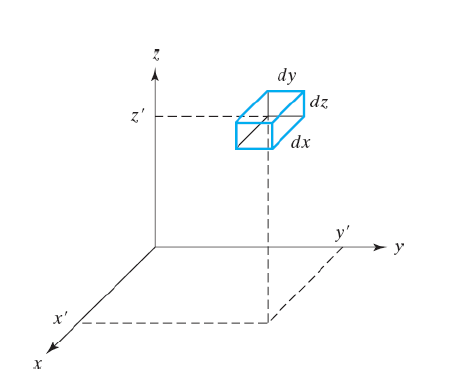
\includegraphics[width=0.5\textwidth]{Figures/3.1.png}  % 图片路径
		\caption{\text{位于}$x^{\prime}, y^{\prime},z^{\prime}$的一个无穷小箱形区域}
		\label{fig:3.1}
	\end{figure}
	虽然(\ref{eq:3.53})看起来很困难,但我们将在第 6 章中解决它。\\
	\indent 对于单粒子一维系统,玻恩假设[式(\ref{exp:1.15 probability of a particle})]表明:$\left|\Psi\left(x^{\prime},t\right)^2\mathrm{d}x\right|$是在$t$时刻在$x^{\prime}$到$x^{\prime}+\mathrm{d}x$区域内找到粒子的概率,其中$x^{\prime}$是$x$的一个特定值。我们对这一假设作如下扩展:\textit{对于三维单粒子系统,表达式}
	\begin{equation}
		\boxed{
			\left|\Psi\left(x^{\prime}, y^{\prime}, z^{\prime},t\right)\right|^2 \mathrm{d}x\mathrm{d}y\mathrm{d}z
		}
		\label{exp:3.54}
	\end{equation}
	\textit{是在$x^{\prime}$到$x^{\prime}+\mathrm{d}x$、$y^{\prime}$到$y^{\prime}+\mathrm{d}y$、$z^{\prime}$到$z^{\prime}+\mathrm{d}z$这一无限小空间内找到粒子的概率。}由于找到粒子的总概率为 1,因此归一化条件为
	\begin{equation}
		\int_{-\infty}^{\infty}\int_{-\infty}^{\infty}\int_{-\infty}^{\infty}\left|\Psi\left(x^{\prime}, y^{\prime}, z^{\prime},t\right)\right|^2 \mathrm{d}x\mathrm{d}y\mathrm{d}z = 1
		\label{eq:3.55}
	\end{equation}
	\indent \textit{对于$n$粒子的三维系统,我们假设}
	\begin{equation}
		\boxed{
			\left|\Psi\left(x_1^{\prime}, y_1^{\prime}, z_1^{\prime},x_2^{\prime}, y_2^{\prime}, z_2^{\prime},\cdots,x_n^{\prime}, y_n^{\prime}, z_n^{\prime},t\right)\right|^2 \mathrm{d}x_1\mathrm{d}y_1\mathrm{d}z_1\mathrm{d}x_2\mathrm{d}y_2\mathrm{d}z_2\cdots\mathrm{d}x_n\mathrm{d}y_n\mathrm{d}z_n
		}
		\label{eq:3.56}
	\end{equation}
	\textit{是在$\left(x_1^{\prime},y_1^{\prime},z_1^{\prime}\right)$处带边$\mathrm{d}x_1,\mathrm{d}y_1,\mathrm{d}z_1$的无限小矩形盒状区域内发现粒子1,在$\left(x_2^{\prime},y_2^{\prime},z_2^{\prime}\right)$处带边$\mathrm{d}x_2,\mathrm{d}y_2,\mathrm{d}z_2$的无限小矩形盒状区域内发现粒子2,$\cdots$,在$\left(x_n^{\prime},y_n^{\prime},z_n^{\prime}\right)$处带边$\mathrm{d}x_n,\mathrm{d}y_n,\mathrm{d}z_n$的无限小矩形盒状区域内发现粒子$n$的概率。}由于找到粒子的总概率为 1,因此归一化条件为
	\begin{equation}
		\int_{-\infty}^{\infty}\int_{-\infty}^{\infty}\int_{-\infty}^{\infty}\cdots\int_{-\infty}^{\infty}\int_{-\infty}^{\infty}\int_{-\infty}^{\infty}\left|\Psi\right|^2 \mathrm{d}x_1\mathrm{d}y_1\mathrm{d}z_1\cdots\mathrm{d}x_n\mathrm{d}y_n\mathrm{d}z_n = 1
		\label{eq:3.57}
	\end{equation}
	\textit{在量子力学中,对一个系统的全空间进行积分的习惯做法是$\int\mathbf{d}\tau$。简写式}(\ref{eq:3.55})\textit{和}(\ref{eq:3.57}),\textit{有}
	\begin{equation}
		\boxed{
			\int\left|\Psi\right|^2\mathrm{d}\tau = 1
		}
		\label{eq:3.58}
	\end{equation}
	\textit{虽然}(\ref{eq:3.58})\textit{看起来像是一个不定积分,但我们可以理解为一个定积分。}根据上下文可以理解积分变量及其范围。\\
	\indent 对于定态系统,$\left|\Psi\right|^2 = \left|\psi\right|^2$,及
	\begin{equation}
		\boxed{
			\int\left|\psi\right|^2\mathrm{d}\tau = 1
		}
		\label{eq:3.59}
	\end{equation}
	
\section{三维盒子中的粒子}
\label{sec:3.5 The Particle in a Three-Dimensional Box}
	目前,我们只讨论单粒子问题。在本节中,我们将考虑第 2.2 节中解决的问题的三维情况,即粒子在盒子中的情况。\\
	\begin{figure}[h!]
		\centering
		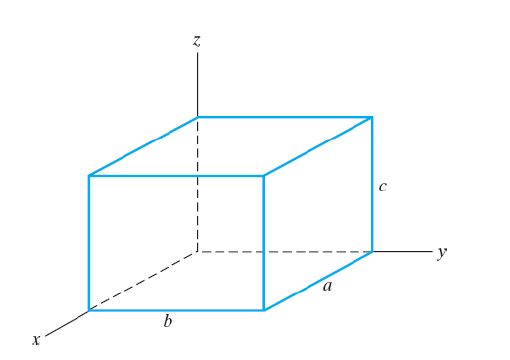
\includegraphics[width=0.5\textwidth]{Figures/3.2.png}  % 图片路径
		\caption{\text{在这个箱形区域内,}$V=0$\text{。}}
		\label{fig:3.2}
	\end{figure}
	\indent 三维盒子有多种可能的形状。我们选择的坐标系使盒子的一个角位于原点,盒子位于空间的第一卦限(图 3.2)。在盒子内,势能为零;而在盒子外,势能为无穷大:
	\begin{equation}
		V\left(x,y,z\right) = 0, \quad \text{其中}
		\begin{cases}
			0 < x < a\\
			0 < y < b\\
			0 < z < c
		\end{cases}
		\label{eq:3.60}
	\end{equation}
	\begin{equation*}
		V = \infty, \quad elsewhere
	\end{equation*}
	\indent 由于粒子具有无限能量的概率为零,因此在盒子外波函数一定为零。在盒内,势能算符为零,薛定谔方程(\ref{eq:3.47})为
	\begin{equation}
		-\frac{\hbar^2}{2m}\left(\frac{\partial^2\psi}{\partial x^2} + \frac{\partial^2\psi}{\partial y^2} + \frac{\partial^2\psi}{\partial z^2}\right) = E\psi
		\label{eq:3.61}
	\end{equation}
	为了求解 (\ref{eq:3.61}),我们假设解可以写成三个分别只与$x$、$y$和$z$有关的单独函数的乘积:
	\begin{equation}
		\psi\left(x,y,z\right) = f\left(x\right)g\left(y\right)h\left(z\right)
		\label{eq:3.62}
	\end{equation}
	我们可能会认为,这一假设抛弃了不满足 (\ref{eq:3.62}) 形式的解。然而,可以证明的是:如果我们能找到满足边界条件的 (\ref{eq:3.62}) 形式的解,那么就不存在满足边界条件的薛定谔方程的其他解了(证明见 G. F. D. Duff 和 D. Naylor, Differential Equations of Applied Mathematics, Wiley, 1966, 第 257-258 页)。我们用来求解 (\ref{eq:3.62}) 的方法称为\textbf{变量分离}(separation of variables)。\\
	\indent 由(\ref{eq:3.62}),我们有
	\begin{equation}
		\frac{\partial^2\psi}{\partial x^2} = f^{\prime\prime}\left(x\right)g\left(y\right)h\left(z\right), \quad \frac{\partial^2\psi}{\partial y^2} = f\left(x\right)g^{\prime\prime}\left(y\right)h\left(z\right)
		\label{eq:3.63}
	\end{equation}
	将(\ref{eq:3.63})和(\ref{eq:3.62})带入式(\ref{eq:3.61}),有
	\begin{equation}
		-\left(\hbar^2/2m\right)f^{\prime\prime}gh-\left(\hbar^2/2m\right)fg^{\prime\prime}h-\left(\hbar^2/2m\right)fgh^{\prime\prime}-Efgh = 0
		\label{eq:3.64}
	\end{equation}
	将上式左右两边同除以$fgh$,有
	\begin{equation}
		- \frac{\hbar^2f^{\prime\prime}}{2mf}- \frac{\hbar^2g^{\prime\prime}}{2mg}- \frac{\hbar^2h^{\prime\prime}}{2mh} -E = 0
		\label{eq:3.65}
	\end{equation}
	\begin{equation}
		-\frac{\hbar^2f^{\prime\prime}\left(x\right)}{2mf\left(x\right)} = \frac{\hbar^2g^{\prime\prime}\left(y\right)}{2mg\left(y\right)}+\frac{\hbar^2h^{\prime\prime}\left(z\right)}{2mh\left(z\right)}+E
		\label{eq:3.66}
	\end{equation}
	\indent 令$E_x$与上式的左边相等,有
	\begin{equation}
		E_x \equiv -\hbar^2f^{\prime\prime}\left(x\right)/2mf\left(x\right)
		\label{eq:3.67}
	\end{equation}
	定义(\ref{eq:3.67})表明$E_x$与$y$和$z$无关,方程(\ref{eq:3.66})表明$E_x$等于$\hbar^2g^{\prime\prime}\left(y\right)/2mg\left(y\right)+\hbar^2h^{\prime\prime}\left(z\right)/2mh\left(z\right)+E$;因此,$E_x$也与$x$无关。综上所述,$E_x$一定是与$x$、$y$和$z$都无关的常数。\\
	\indent 与(\ref{eq:3.67})类似,我们定义$E_y$与$E_z$:
	\begin{equation}
		E_y \equiv -\hbar^2g^{\prime\prime}\left(y\right)/2mf\left(y\right), \quad E_z \equiv -\hbar^2h^{\prime\prime}\left(z\right)/2mh\left(z\right)
		\label{eq:3.68}
	\end{equation}
	由于 $x$、$y$、$z$ 在 (\ref{eq:3.65}) 中对称出现,因此与证明 $E_x$ 是常数的推理相同,$E_y$ 和 $E_z$ 也是常数。将定义(\ref{eq:3.67})和(\ref{eq:3.68})代入(\ref{eq:3.65})可得
	\begin{equation}
		E_x+E_y+E_z=E
		\label{eq:3.69}
	\end{equation}
	\indent 方程(\ref{eq:3.67})和(\ref{eq:3.68})为
	\begin{equation}
		\frac{\mathrm{d}^2f\left(x\right)}{\mathrm{d}x^2}+\frac{2m}{\hbar^2}E_xf\left(x\right) = 0
		\label{eq:3.70}
	\end{equation}
	\begin{equation}
		\frac{\mathrm{d}^2g\left(y\right)}{\mathrm{d}y^2}+\frac{2m}{\hbar^2}E_yg\left(y\right) = 0, \quad \frac{\mathrm{d}^2h\left(z\right)}{\mathrm{d}z^2}+\frac{2m}{\hbar^2}E_zh\left(z\right) = 0
		\label{eq:3.71}
	\end{equation}
	我们已将三变量的偏微分方程转换为三个常微分方程。(\ref{eq:3.70}) 的边界条件是什么?由于波函数在盒外消失,因此连续性要求波函数$\psi$在盒壁处消失。特别是,在 $yOz$ 平面上的盒壁上必须为零,此处$x=0$;此外,在箱体的平行壁上必须为零,其中$x=a$。因此,$f\left(0\right) = f\left(a\right) = 0$。\\
	\indent 现在将公式 (\ref{eq:3.70}) 与一维盒子中粒子的薛定谔方程 [公式 (\ref{eq:2.10 schrödinger equation for particle between 0 and l}) ] 进行比较。方程的形式相同,(\ref{eq:3.70}) 中的 $E_x$ 与 (\ref{eq:2.10 schrödinger equation for particle between 0 and l}) 中的 $E$ 相对应。边界条件是否相同?是的,只是自变量消失的第二点是 $x=a$,而不是 $x=l$。因此,我们可以利用第 2.2 节中的工作来写出解[见式 (\ref{eq:2.23 stationary state wave function for the particle in a box}) 和 (\ref{eq:2.20 energy of one-dimensional box}) ]。
	\begin{equation*}
		f\left(x\right) = \left(\frac{2}{a}\right)^{1/2}\sin\left(\frac{n_x\pi x}{a}\right)
	\end{equation*}
	\begin{equation*}
		E_x = \frac{n_x^2h^2}{8ma^2}, \quad n_x = 1,2,3\cdots
	\end{equation*}
	将同样的推理应用于 $y$ 和 $z$ 方程,可以得出
	\begin{equation*}
		g\left(y\right) = \left(\frac{2}{b}\right)^{1/2}\sin\left(\frac{n_y\pi y}{b}\right), \quad h\left(z\right) = \left(\frac{2}{c}\right)^{1/2}\sin\left(\frac{n_z\pi z}{c}\right)
	\end{equation*}
	\begin{equation*}
		E_y = \frac{n_y^2h^2}{8mb^2}, \quad n_x = 1,2,3\cdots, \quad E_z = \frac{n_z^2h^2}{8mc^2}, \quad n_z = 1,2,3\cdots
	\end{equation*}
	\indent 由(\ref{eq:3.69}),能量为
	\begin{equation}
		E = \frac{h^2}{8m}\left(\frac{n_x^2}{a^2}+\frac{n_y^2}{b^2}+\frac{n_z^2}{c^2}\right)
		\label{eq:3.72}
	\end{equation}
	与一维盒子中的粒子一样,基态能量大于经典力学的最低能量值0。\\
	\indent 由式(\ref{eq:3.62}),箱中粒子的波函数为
	\begin{equation}
		\psi\left(x,y,z\right) = \left(\frac{8}{abc}\right)^{1/2}\sin\left(\frac{n_x\pi x}{a}\right)\sin\left(\frac{n_y\pi y}{b}\right)\sin\left(\frac{n_z\pi z}{c}\right)
		\label{eq:3.73}
	\end{equation}
	\indent 波函数有三个量子数$n_x$、$n_y$和$n_z$,我们将其归因于问题的三维性质。三个量子数彼此独立变化。\\
	\indent 在一维单粒子问题中,节点满足$\psi\left(x\right)=0$,解这个方程,我们就得到了$\psi = 0$的$x$值。而在三维单粒子问题中,节点满足$\psi\left(x,y,z\right) = 0$,从方程中解出$z$,我们有$z=f\left(x,y\right)$,每个这样的解都是三维空间中一个\textbf{节面}(nodal surface)的方程。例如,对于$n_x=1$、$n_y=1$、$n_z=2$的定态,令波函数($\ref{eq:3.73}$)为0,解得节面为$z=c/2$,这是一个平面的方程,该平面平行于盒子的顶面和底面,并且位于这两个面的中间。同样地,对于状态$n_x=2$、$n_y=1$、$n_z=1$,节面为$x=a/2$的平面。\\
	\indent 由于波函数中的$x$、$y$和$z$因子可以独立归一化,将波函数归一化,有
	\begin{equation*}
		\int_{-\infty}^{\infty}\int_{-\infty}^{\infty}\int_{-\infty}^{\infty}\left|\psi\right|^2\mathrm{d}x\mathrm{d}y\mathrm{d}z = \int_{0}^{a}\left|f\left(x\right)\right|^2\mathrm{d}x\int_{0}^{b}\left|g\left(y\right)\right|^2\mathrm{d}y\int_{0}^{c}\left|h\left(z\right)\right|^2\mathrm{d}z=1
	\end{equation*}
	其中我们用到了
	\begin{equation}
		\boxed{
			\int\int\int F\left(x\right)G\left(y\right)H\left(z\right)\mathrm{d}x\mathrm{d}y\mathrm{d}z = \int F\left(x\right)\mathrm{d}x\int G\left(y\right)\mathrm{d}y\int H\left(z\right)\mathrm{d}z
		}
		\label{eq:3.74}
	\end{equation}
	\indent 式(\ref{eq:3.73})中$\psi\left(x,y,z\right)$的量纲是什么?对于单粒子三维系统,$\left|\psi\right|^2\mathrm{d}x\mathrm{d}y\mathrm{d}z$是概率,概率是没有量纲的。由于$\mathrm{d}x\mathrm{d}y\mathrm{d}z$的量纲为长度$^3$,则为了使$\left|\psi\right|^2\mathrm{d}x\mathrm{d}y\mathrm{d}z$无量纲,$\psi\left(x,y,z\right)$一定具有长度$^{-3/2}$的量纲。\\
	\indent 假设$a=b=c$,则我们得到了一个立方体。能级为
	\begin{equation}
		E = \left(h^2/8ma^2\right)\left(n_x^2+n_y^2+n_z^2\right)
		\label{eq:3.75}
	\end{equation}
	让我们用表格列出被限制在立方体势箱中粒子的一些允许能量:
	\begin{equation*}
		\begin{array}{c|c|c|c|c|c|c|c|c|c|c|c}
			n_xn_yn_z & 111 & 211 & 121 & 112 & 122 & 212 & 221 & 113 & 131 & 311 & 222 \\
			\hline E\left(8ma^2/h^2\right) & 3 & 6 & 6 & 6 & 9 & 9 & 9 & 11 & 11 & 11 & 12
		\end{array}
	\end{equation*}
	\begin{figure}[h!]
		\centering
		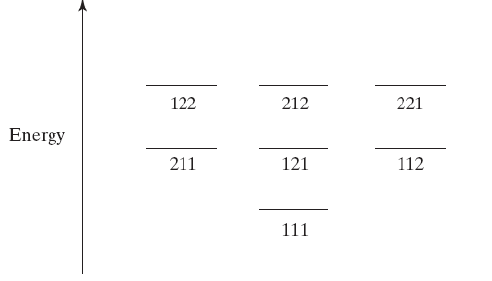
\includegraphics[width=0.5\textwidth]{Figures/3.3.png}  % 图片路径
		\caption{\text{立方体盒子中粒子最低几个状态的能量。}}
		\label{fig:3.3}
	\end{figure}
	\\
	\indent 请注意:量子数不同的状态可能具有相同的能量(图\ref{fig:3.3})。例如,状态$\psi_{211}$、$\psi_{121}$和$\psi_{112}$(下标表示量子数)都具有相同的能量。然而,公式 (\ref{eq:3.73}) 表明这三组量子数给出了三个不同的独立波函数,因此确实代表了系统的不同状态。当两个或两个以上的独立波函数对应于具有相同能量本征值的状态时,该本征值是\textbf{简并}(degenerate)的。一个能级的\textbf{简并度}(degree of degeneracy or simply degeneracy)就是具有该能量的状态的数量。因此,立方体中粒子的次低能级是三重简并的。当我们令盒子的边长相等时,就得到了简并的现象。简并度通常与系统的对称性有关。注意波函数态$\psi_{211}$、$\psi_{121}$和$\psi_{112}$可以通过旋转立方体盒相互转化。通常,一维问题中的束缚态能级是非简并的。\\
	\indent 在对理想气体的分子分配函数进行统计力学评估时,将每个气体分子的平移能级视为三维矩形盒子(盒子是容纳气体的容器)中的粒子能级;见Levine,《物理化学》,第 21.6 和 21.7 节。\\
	\indent 在金属的自由电子理论中,非过渡金属的价电子被视为一个盒子中的非相互作用粒子,盒子的两侧是金属的表面。这种近似方法虽然粗糙,但对金属的某些性质给出了相当不错的结果。
	
\section{简并}
\label{sec:3.6 Degeneracy}
	对于一个$n$重简并的能级,有$n$个独立的波函数$\psi_1$,$\psi_2$,$\psi_3$,$\cdots$,$\psi_n$每个波函数均有本征值$w$:
	\begin{equation}
		\hat{H}\psi_1 = w\psi_1, \quad\hat{H}\psi_2 = w\psi_2, \cdots,\quad \hat{H}\psi_n = w\psi_n
		\label{eq:3.76}
	\end{equation}
	我们想要证明以下重要理论:\textit{具有能量本征值 $w$ 的简并波函数的每一个线性组合}
	\begin{equation}
		\phi \equiv c_1\psi_1 + c_2\psi_2 + c_3\psi_3 + \cdots + c_n\psi_n
		\label{eq:3.77}
	\end{equation}
	\textit{也是能量本征函数,且具有相同的能量本征值 $w$。} [式(\ref{eq:3.77})是函数$\psi_1$,$\psi_2$,$\psi_3$,$\cdots$,$\psi_n$\textbf{线性组合}的定义。其中$c$是常数,有些可能为零。]为了证明这个理论,我们必须指明$\hat{H}\phi = w\phi$,或者
	\begin{equation}
		\hat{H}\left(c_1\psi_1 + c_2\psi_2 +  \cdots + c_n\psi_n\right) = w\left(c_1\psi_1 + c_2\psi_2 + \cdots + c_n\psi_n\right)
		\label{eq:3.78}
	\end{equation}	
	由于$\hat{H}$是线性算符,我们可以对式(\ref{eq:3.78})的左边应用式(\ref{eq:3.9})$n-1$次,有
	\begin{equation*}
		\hat{H}\left(c_1\psi_1 + c_2\psi_2 +  \cdots + c_n\psi_n\right) = \hat{H}\left(c_1\psi_1\right) + \hat{H}\left(c_2\psi_2\right) + \cdots + \hat{H}\left(c_n\psi_n\right)
	\end{equation*}
	再使用式(\ref{eq:3.10}),则(\ref{eq:3.79})变为
	\begin{equation*}
		\begin{aligned}
			\hat{H}\left(c_1\psi_1 + c_2\psi_2 +  \cdots + c_n\psi_n\right) &= c_1\hat{H}\psi_1 + c_2\hat{H}\psi_2 +  \cdots + c_n\hat{H}\psi_n \\
			&= c_1w\psi_1 + c_2w\psi_2 +  \cdots + c_nw\psi_n \\
			\hat{H}\left(c_1\psi_1 + c_2\psi_2 +  \cdots + c_n\psi_n\right) &= w\left(c_1\psi_1 + c_2\psi_2 +  \cdots + c_n\psi_n\right)
		\end{aligned}
	\end{equation*}
	这就证明了我们的理论。\\
	\indent 例如,在立方势箱中粒子的定态波函数$\psi_{211}$、$\psi_{121}$和$\psi_{112}$是简并的,则它们的线性组合$c_1\psi_{211} + c_2\psi_{121} + c_3\psi_{112}$立方势箱中粒子哈密顿算符的本征函数,且具有相同的能量本征值$6h^2/8ma^2$,与$\psi_{211}$、$\psi_{121}$和$\psi_{112}$相同。\\
	\indent 注意:若$\psi_1$和$\psi_2$对应于不同的能量本征值($\hat{H}\psi_1 = E_1\psi_1$,$\hat{H}\psi_2 = E_2\psi_2$,且$E_1 \neq E_2$),则它们的线性组合$c_1\psi_1+c_2\psi_2$不是能量算符$\hat{H}$的本征函数。\\
	\indent 由于与简并能级相对应的波函数的任何线性组合都是具有相同本征值的 $\hat{H}$ 的本征函数,因此我们可以为任何简并能级构造出无数个不同的波函数。事实上,我们只对线性无关的本征函数感兴趣。若$f_1,f_2,\cdots,f_n$当且仅当所有常数$c_1,c_2,\cdots,c_n$都为零时,满足关系式$c_1f_1+c_2f_2+\cdots+c_nf_n=0$,则称$f_1,f_2,\cdots,f_n$是\textbf{线性无关}的。这就意味着\textit{在一组线性独立函数中,没有一个函数可以用其余函数的线性组合来表示。}例如,函数$f_1=3x$,$f_2=5x^2-x$,$f_3=x^2$不是线性无关的,因为$f_2=5f_3-\frac{1}{3}f_1$。而函数$g_1=1$,$g_2=x$,$g_3=x^2$是线性无关的,因为没有一个函数可以用其余函数的线性组合来表示。\\
	\indent 一个能级的\textbf{简并度}等于与该能值相对应的线性独立波函数的数目。一维自由粒子波函数 (\ref{eq:2.30}) 是两个线性独立函数的线性组合,这两个函数分别是具有相同能量本征值 $E$ 的本征函数。因此每个这样的能级(除了$E=0$)都是二重简并的(简并度为2)。\\

\section{平均值}
\label{sec:3.7 Average Values}
	第3.3节指出:若态函数$\Psi$不是算符$\hat{B}$的本征函数,则对$B$的观测将得到一组可能值($\hat{B}$的本征值的其中一个)。我们现在考虑具有状态$\Psi$的系统的性质$B$的平均值。\\
	\indent 为了在实验中找到 $B$ 的平均值,我们需要许多相同的、不相互影响的系统$\Psi$,每个系统都处于相同的状态,然后测量每个系统中的 $B$。$B$的\textbf{平均值}(average value),记作$\langle B \rangle$,定义为所有测量值$b_1,b_2,\cdots,b_N$的算术平均:
	\begin{equation}
		\langle B \rangle = \frac{1}{N}\sum_{j=1}^{N}B_j
		\label{eq:3.79}
	\end{equation}
	其中系统的数目$N$是很大的一个数。\\
	\indent 我们可以对 $B$ 的所有可能值求和,而不是对 $B$ 的观测值求和,将每个可能值乘以观测到的次数,得到等价表达式
	\begin{equation}
		\langle B \rangle = \frac{1}{N}\sum_{b}n_bb
		\label{eq:3.80}
	\end{equation}
	其中 $n_b$ 是观测到的值 $b$ 的次数。举一个例子就会很清楚。假设一个班级的五名学生进行了五道题的测试,取得的分数为:0,20,20,60,60,80,80,80,100。则用式(\ref{eq:3.79})计算平均分,我们有
	\begin{equation*}
		\frac{1}{N}\sum_{j=2}^{N}B_j = \frac{0+20+20+60+60+80+80+80+100}{9} = \frac{500}{9} = 56
	\end{equation*}
	用式(\ref{eq:3.80})计算平均分,对所有可能的分数:0,20,40,60,80,100求和,我们有
	\begin{equation*}
		\frac{1}{N}\sum_{b}n_bb = \frac{1\left(0\right)+2\left(20\right)+0\left(40\right)+2\left(60\right)+3\left(80\right)+1\left(100\right)}{9} = \frac{500}{9} = 56
	\end{equation*}
	\indent 方程(\ref{eq:3.80})可以写作
	\begin{equation*}
		\langle B \rangle = \sum_{b}\left(\frac{n_b}{N}\right)b
	\end{equation*}
	由于$N$很大,$n_b/N$是观测到值$b$的概率$P_b$,因此
	\begin{equation}
		\langle B \rangle = \sum_{b}P_bb
		\label{eq:3.81}
	\end{equation}
	\indent 现在考虑态函数为$\Psi\left(x,t\right)$的一维单粒子系统中$x$坐标的平均值。$x$ 坐标的取值范围是连续的,在$x$到$x+\mathrm{d}x$的无限小区间内找到粒子的概率为$\left|\Psi\right|^2\mathrm{d}x$。对无限小区间的求和等同于对整个 $x$ 范围的积分,因此 (\ref{eq:3.81}) 变为
	\begin{equation}
		\langle x \rangle = \int_{-\infty}^{\infty}x\left|\Psi\left(x,t\right)\right|^2\mathrm{d}x
		\label{eq:3.82}
	\end{equation}
	对于单粒子三维系统,在位于$\left(x,y,z\right)$,具有边长$\mathrm{d}x,\mathrm{d}y,\mathrm{d}z$的体积微元内找到粒子的概率为
	\begin{equation}
		\left|\Psi\left(x,y,z,t\right)\right|^2\mathrm{d}x\mathrm{d}y\mathrm{d}z
		\label{eq:3.83}
	\end{equation}
	如果我们想知道在$x$到$x+\mathrm{d}x$的范围内找到粒子的概率,我们必须用$y$和$z$的所有可能取值对式(\ref{eq:3.83})进行积分,由于当$x$在$x+\mathrm{d}x$范围内时,粒子的$y$和$z$坐标可以任意取值。因此,对于三维的例子,式(\ref{eq:3.82})变为
	\begin{equation}
		\langle x \rangle = \int_{-\infty}^{\infty}\left[\int_{-\infty}^{\infty}\int_{-\infty}^{\infty}\left|\Psi\left(x,y,z,t\right)\right|^2\mathrm{d}y\mathrm{d}z\right]x\mathrm{d}x
		\label{eq:3.84}
	\end{equation}
	\begin{equation*}
		\langle x \rangle = \int_{-\infty}^{\infty}\int_{-\infty}^{\infty}\int_{-\infty}^{\infty}x\left|\Psi\left(x,y,z,t\right)\right|^2\mathrm{d}x\mathrm{d}y\mathrm{d}z
	\end{equation*}
	\indent 现在,我们来看看某种物理特性 $B\left(x,y,z\right)$ 的平均值,它是粒子坐标的函数。一个例子就是势能函数$V\left(x,y,z\right)$。根据式 (\ref{eq:3.84}) 的相同推理,可以得出
	\begin{equation}
		\langle B\left(x,y,z\right) \rangle = \int_{-\infty}^{\infty}\int_{-\infty}^{\infty}\int_{-\infty}^{\infty}\left|\Psi\left(x,y,z,t\right)\right|^2B\left(x,y,z\right)\mathrm{d}x\mathrm{d}y\mathrm{d}z
		\label{eq:3.85}
	\end{equation}
	\begin{equation}
		\langle B\left(x,y,z\right) \rangle = \int_{-\infty}^{\infty}\int_{-\infty}^{\infty}\int_{-\infty}^{\infty}\Psi^{\ast}B\Psi\mathrm{d}x\mathrm{d}y\mathrm{d}z
		\label{eq:3.86}
	\end{equation}
	式(\ref{eq:3.86}) 的形式似乎有点异想天开,因为它与 (\ref{eq:3.85}) 没有什么不同。但稍后我们将看到它的重要意义。\\
	\indent 一般来说,对于单粒子三维系统,属性 $B$ 既取决于坐标,也取决于动量:
	\begin{equation*}
		B = B\left(x,y,z,p_x,p_y,p_z\right)
	\end{equation*}
	我们如何找到$B$的平均值?我们\textit{假设}处于$\Psi$状态的系统的$\langle B \rangle$为
	\begin{equation*}
		\langle B \rangle = \int_{-\infty}^{\infty}\int_{-\infty}^{\infty}\int_{-\infty}^{\infty}\Psi^{\ast}B\left(x,y,z,\frac{\hbar^2}{\mathrm{i}}\frac{\partial}{\partial x},\frac{\hbar^2}{\mathrm{i}}\frac{\partial}{\partial y},\frac{\hbar^2}{\mathrm{i}}\frac{\partial}{\partial z}\right)\Psi\mathrm{d}x\mathrm{d}y\mathrm{d}z
	\end{equation*}
	\begin{equation}
		\langle B \rangle = \int_{-\infty}^{\infty}\int_{-\infty}^{\infty}\int_{-\infty}^{\infty}\Psi^{\ast}\hat{B}\Psi\mathrm{d}x\mathrm{d}y\mathrm{d}z
		\label{eq:3.87}
	\end{equation}
	其中$\hat{B}$是性质$B$的量子力学算符。[稍后,我们将利用 (\ref{eq:3.87}) 来证明含时薛定谔方程在从量子力学到经典力学的转变过程中还原为牛顿第二定律,从而为这一假设提供一些理由;见问题 7.59。],对于$n$粒子体系,我们假设
	\begin{equation}
		\boxed{
			\langle B \rangle = \int \Psi^{\ast}\hat{B}\Psi\mathrm{d}\tau
		}
		\label{eq:3.88}
	\end{equation}
	其中$\int\mathrm{d}\tau$表示对全空间的$3n$坐标的积分。由于我们将$\Psi^{\ast}\Psi$视为概率密度,式(\ref{eq:3.88})中的态函数必须先归一化。重要的是,要将算符放在在$\Psi^{\ast}$和$\Psi$中间。表达式$\hat{B}\Psi^{\ast}\Psi$、$\Psi^{\ast}\Psi\hat{B}$和$\Psi^{\ast}\hat{B}\Psi$的含义是不同的,除非$B$只是坐标的函数。在$\int\Psi^{\ast}\hat{B}\Psi\mathrm{d}\tau$中,第一个操作是将算符$\hat{B}$应用于态函数$\Psi$,然后将结果与$\Psi^{\ast}$相乘并对全空间进行积分,就得到了$\langle B \rangle$。\\
	\indent 对于定态,我们有[式\ref{eq:1.20}]
	\begin{equation*}
		\Psi^{\ast}\hat{B}\Psi = \mathrm{e}^{\mathrm{i}Et/\hbar}\psi^{\ast}\hat{B}\mathrm{e}^{-\mathrm{i}Et/\hbar}\psi = \mathrm{e}^{0}\psi^{\ast}\hat{B}\psi = \psi^{\ast}\hat{B}\psi
	\end{equation*}
	由于$\hat{B}$不包含对时间的导数,也不会影响 $\Psi$ 中的时间因子,因此,对于定态,有
	\begin{equation}
		\langle B \rangle = \int \psi^{\ast}\hat{B}\psi\mathrm{d}\tau
		\label{eq:3.89}
	\end{equation}
	因此,在定态系统中,若$\hat{B}$与时间无关,则$\langle B \rangle$也是与时间无关的。\\
	\indent 考虑一个特殊的例子,若$\Psi$是$\hat{B}$的本征函数。当$\hat{B}\Psi = k\Psi$时,式(\ref{eq:3.88})变为
	\begin{equation*}
		\langle B \rangle = \int \Psi^{\ast}\hat{B}\Psi\mathrm{d}\tau = \int \Psi^{\ast}k\Psi\mathrm{d}\tau = k \int \Psi^{\ast}\Psi\mathrm{d}\tau = k
	\end{equation*}
	其中$\Psi$已归一化。由于当$\hat{B}\Psi = k\Psi$时,$k$ 是我们在测量时能找到的唯一可能的 $B$ 值,因此这个结果是合理的(第 3.3 节)。\\
	\indent 由式(\ref{eq:3.88})很容易证明以下关于平均值的性质(见问题 3.49):
	\begin{equation}
		\boxed{
			\langle A + B \rangle = \langle A \rangle + \langle B \rangle
		}
		\quad
		\boxed{
			\langle cB \rangle = c\langle B \rangle
		}
		\label{eq:3.90}
	\end{equation}
	其中$A$和$B$是系统的物理量,$c$是常数。但是,平均值的乘积不一定等于乘积的平均值:$\langle AB \rangle \neq \langle A \rangle\langle B \rangle$。\\
	\indent 通常使用\textbf{期望值}(expectation value)一词来代替平均值。期望值并不一定是我们观察到的可能值之一。
	\begin{examplebox}
		\textbf{例题:}对于处于基态的三维单粒子系统,求$\langle x \rangle$和$\langle p_x \rangle$的值。\\
		\\
		将基态波函数$\psi=f\left(x\right)g\left(y\right)h\left(z\right)$[式(\ref{eq:3.62})]代入式(\ref{eq:3.89}),有
		\begin{equation*}
			\langle x \rangle = \int \psi^{\ast}\hat{x}\psi \mathrm{d}\tau = \int_{0}^{c}\int_{0}^{b}\int_{0}^{a}f^{\ast}g^{\ast}h^{\ast} x fgh\mathrm{d}x\mathrm{d}y\mathrm{d}z
		\end{equation*}
		而在势箱外有$\psi = 0$。由于$g\left(y\right)$和$h\left(z\right)$已归一化,使用式(\ref{eq:3.74}),我们有
		\begin{equation*}
			\langle x \rangle = \int_{0}^{a} x\left|f\left(x\right)\right|^{2}\mathrm{d}x \int_{0}^{b}\left|g\left(y\right)\right|^{2}\mathrm{d}y \int_{0}^{c}\left|h\left(z\right)\right|^{2}\mathrm{d}z = \int_{0}^{a} x\left|f\left(x\right)\right|^{2}\mathrm{d}x
		\end{equation*}
		由于系统处于基态,有$n_x=1$,则$f\left(x\right) = \left(2/a\right)^{1/2}\sin\left(\pi x/a\right)$,因此
		\begin{equation}
			\langle x \rangle = \frac{2}{a}\int_{0}^{a} x\sin^{2}\left(\frac{\pi x}{a}\right)\mathrm{d}x = \frac{a}{2}
			\label{eq:3.91}
		\end{equation}
		其中我们用到了附录中的(A.3)。根据图\ref{fig:2.4},这个结果是合理的。\\
		\indent 同样地,
		\begin{equation*}
			\langle p_x \rangle = \int \psi^{\ast}\hat{p}_x\psi \mathrm{d}\tau = \int_{0}^{c}\int_{0}^{b}\int_{0}^{a}f^{\ast}g^{\ast}h^{\ast} \frac{\hbar}{\mathrm{i}}\frac{\partial}{\partial x}\left[f\left(x\right)g\left(y\right)h\left(z\right)\right]\mathrm{d}x\mathrm{d}y\mathrm{d}z
		\end{equation*}
		\begin{equation*}
			\langle p_x \rangle = \frac{\hbar}{\mathrm{i}}\int_{0}^{a}f^{\ast}\left(x\right)f^{\prime}\left(x\right)\mathrm{d}x \int_{0}^{b}\left|g\left(y\right)\right|^{2}\mathrm{d}y \int_{0}^{c}\left|h\left(z\right)\right|^{2}\mathrm{d}z
		\end{equation*}
		\begin{equation}
			\langle p_x \rangle = \frac{\hbar}{\mathrm{i}}\int_{0}^{a}f\left(x\right)f^{\prime}\left(x\right)\mathrm{d}x = \frac{\hbar}{2\mathrm{i}}\left. f^2\left(x\right) \right|_{0}^{a} = 0
			\label{eq:3.92}
		\end{equation}
		其中,我们用到了定解条件$f\left(0\right)=f\left(a\right)=0$。由于粒子向$+x$和$-x$方向的移动是等概率的,因此这个结果是合理的。\\
		\\
		\textbf{练习:}求处于基态的三维单粒子系统的$\langle p_x^2 \rangle$的值。\\
		(\textit{答案:}$h^2/4l^2$。)
	\end{examplebox}

\section{波函数的约束条件}
\label{sec:3.8 Requirements for an Acceptable Wave Function}
	在求解箱中粒子的问题时,我们要求$\psi$是连续的。我们现在讨论波函数需要满足的其他约束条件。\\
	\indent 由于$\left|\psi\right|^2\mathrm{d}\tau$是概率,我们希望可以通过选择一个合适的\textbf{归一化常数}(normalization constant)与波函数相乘,使得波函数可以归一化。若$\psi$未归一化而$N\psi$已归一化,则根据归一化条件,有
	\begin{equation}
		1 = \int \left|N\psi\right|^2\mathrm{d}\tau = N^2\int \left|\psi\right|^2\mathrm{d}\tau
		\label{eq:3.93}
	\end{equation}
	\begin{equation*}
		N = \left(\int \left|\psi\right|^2\mathrm{d}\tau\right)^{-1/2}
	\end{equation*}
	\begin{figure}[h!]
		\centering
		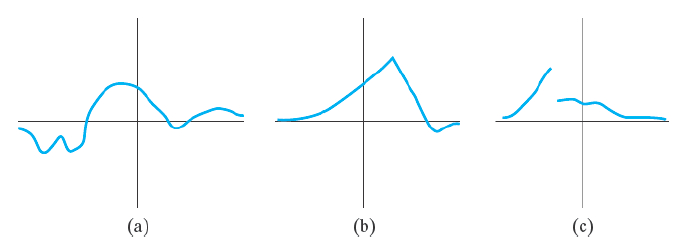
\includegraphics[width=0.5\textwidth]{Figures/3.4.png}  % 图片路径
		\caption{\shortstack{\text{函数(a)是连续函数,其一阶导数也连续;}\\\text{函数(b)是连续函数,但其一阶导数不连续;}\\\text{函数(c)不是连续函数}}}
		\vspace{-6pt}
		\label{fig:3.4}
	\end{figure}
	只有当$\psi$处处为零时,定积分$\int \left|\psi\right|^2\mathrm{d}\tau$才为零。然而,$\psi$不可能处处为零(这意味着没有粒子存在)。因此,这个积分一定不会为零。若$\int \left|\psi\right|^2\mathrm{d}\tau$为无穷大,则$\left|N\right|$为零,$\psi$就无法归一化。当且仅当$\int \left|\psi\right|^2\mathrm{d}\tau$具有有限而非无限值时,我们才能对$\psi$进行归一化。如果对全空间的积分$\int \left|\psi\right|^2\mathrm{d}\tau$为有限值,我们说$\psi$是\textbf{平方可积的}(quadratically integrable)。因此,我们一般要求$\psi$是平方可积的。一个最重要的例外不处于束缚态的粒子。因此,粒子在势阱中(第 2.4 节)的非束缚态和自由粒子的波函数都不是平方可积的。\\
	\indent 由于$\psi^{\ast}\psi$是概率密度,因此波函数一定是单值的。如果我们的理论对在某一点发现粒子的概率给出了两个不同的值,那就太尴尬了。如果我们要求$\psi$是单值的,那么显然$\psi^{\ast}\psi$也是单值的。$\psi$可能会有多个值[例如,$\psi\left(q\right) = -1,1,\mathrm{i}$],但$\psi^{\ast}\psi$只能有一个值。然而,我们仍要求$\psi$是单值的。\\
	\indent 除了要求$\psi$是连续,我们也通常要求其偏导数$\partial\psi/\partial x$,$\partial\psi/\partial y$等也是连续的(见图\ref{fig:3.4}a)。不过,回过头来看第 2.2 节,我们会发现:对于箱中粒子$\partial\psi/\partial x$在箱壁上不连续,以及$\partial\psi/\partial x$在箱外为零,但是由方程(\ref{eq:2.23 stationary state wave function for the particle in a box})可知,$\partial\psi/\partial x$在箱壁上又不为零。$\psi^{\prime}$的不连续性是由在箱壁处势能突然变为无穷大造成的。对于具有有限高度的势垒来说,$\psi^{\prime}$在箱壁处是连续的。\\
	\indent 与平方可积的要求一致,有时也会说波函数必须在任何地方都是有限的,包括无穷大。然而,这通常是比平方可积性更强的要求。事实上,氢原子的一些相对论波函数在原点处是无限的,但却是平方可积的。偶尔,我们也会遇到在原点处无限大的非相对论波函数 [L. D.D. 兰道和 E. M. 利夫希茨,《量子力学》,第三版(1977 年),第 35 节]。因此,基本要求是平方可积性,而不是有限性。\\
	\indent 我们要求任何代表物理量的算符的本征函数都满足上述要求。符合这些要求的函数被称为\textbf{品优函数}(well-behaved function)。

\section*{总结}

\section*{习题}